\section{One dimentional fit and mass resolution}

For the nominal results, 
the relativistic Breit-Wigner function (BW) of free pole mass ($M$) and width ($\Gamma$) is used for the signal shape:

\begin{equation}
	BW(m|M,\Gamma) = \frac{B_{p}B_{q}} { \frac{M^{2}-m^{2}}{M\Gamma} - i} 
	\times \frac{1}{\sqrt{\pi \frac{\Gamma}{2}} I}  
\end{equation}
where $B_{p}$, $B_{q}$ are optional Blatt-Weisskopf factors
(the nominal fits assume S-wave production and decay, thus $B_{p}$ = $B_{q}$ = 1) 
and I is the normalization integral. 
The definition of $I$ affects only the signal yield convention, and is given by:

\begin{equation}
	I = \frac{1}{\pi} ( arctan( \frac{m_{max}-M} { \frac{\Gamma}{2} } ) 
		- arctan( \frac{m_{min}-M} { \frac{\Gamma}{2} } )
\end{equation}
where $[m_{min},m_{max}]$ is the fit range. 
The latter is an accurate integral of the magnitude ($|BW|^2$) of non-relativistic Breit-Wigner function, in which

\begin{equation}
	\frac{M^{2}-m^{2}}{M\Gamma} \to \frac{M-m}{\frac{\Gamma}{2}}
\end{equation}
This formula is surprisingly accurate for the relativistic Breit-Wigner as well,
especially when the fit boundaries are far from the pole mass as measured in units of the width. 
As seen from the equations above, we use mass-independent resonant width. 
We have checked that considering its mass dependence ($\Gamma\to\Gamma(m)=\Gamma\frac{q}{q_{0}}\frac{M}{m}B_{q}^{2}$) 
has negligible effect on our fits results, since the signal peaks are narrow.
Besides,
the Blatt-Weisskopf  factor used here is similar to the one mentioned in $\Bp\to\jpsi\phi\Kp$ amplitude analysis.


We use polynomial functions ($pol$) of various order to describe the smooth background 
under the $P_{c}^+$ peaks ($\Lb\to\jpsi\Lz^{*}$ is the main background source). 
The polynomial coefficients are free fit parameters. 
Switching from the plain to Chebyshev polynomials improved numerical stability of the fits for high orders of the polynomial:

%\begin{equation}
%	pol(m|\vec{a}) = \sum_{n=0}^{N_{{pol}} a_{nb} T_{n}(x_{m})   \\
%	x_{m} = 2 \frac{m-m_{min}}{m_{max}-m_{max}} -1 \\
%	T_{0}(x_m) = 1, T_{1}(x_m) = x_{m}, T_{n+1}(x_m) = 2x_{m} T_{n}(x_m) - T_{n-1}(x_m)
%\end{equation}
The Chebyshev polynomials ($T_{n}$) are orthogonal to each other, 
when the fit range is mapped to the $[−1, +1]$ range (the $x_m$ variable). 
This reduces correlations between the fitted polynomial coefficients, 
making convergence faster and avoiding round-off problems in the calculation of the covariance matrix.

The phase-space factor, $pq$, 
multiplies the signal and background functions added together, 
where $p(q)$ is the $P_c^+(\jpsi)$ momentum in the \Lb ($P_c^+$) rest frame. 
This factor is always included, 
even if we don’t explicitly mention it in the figure captions.
When overlapping signal peaks are fitted, 
we first add them incoherently when constructing the PDF function ($P$):

\begin{equation}
	P(m) = p \dot q ( \sum_{j} Y_{j} |BW(m|M_j,\Gamma_j)|^2 + pol(m|\vec{a}))
\end{equation}
When allowing for their interference, 
a relative complex phase $\delta_j$ is added as a free parameter:

\begin{equation}
	| \sum_{j=1} \sqrt{|Y_j|} e^{i\delta_j} BW(m|M_j,\Gamma_j) |^2
	P(m) = p \dot q ( \sum_{j} Y_{j} |BW(m|M_j,\Gamma_j)|^2 + pol(m|\vec{a}))
\end{equation}
We parameterize the observed $m_{jpsi\proton}$ dependence with a quadratic function, $\sigma_m(m)$, 
as shown in Figure.~\ref{}, 
and smear any fit function with a Gaussian of appropriate width:
\begin{equation}
   P_{smeared}(m) = \sum_{k} P_{k} P(m+x_{k}\sigma_{m}(m))
\end{equation}

\begin{figure}[!hbtp]
\centering
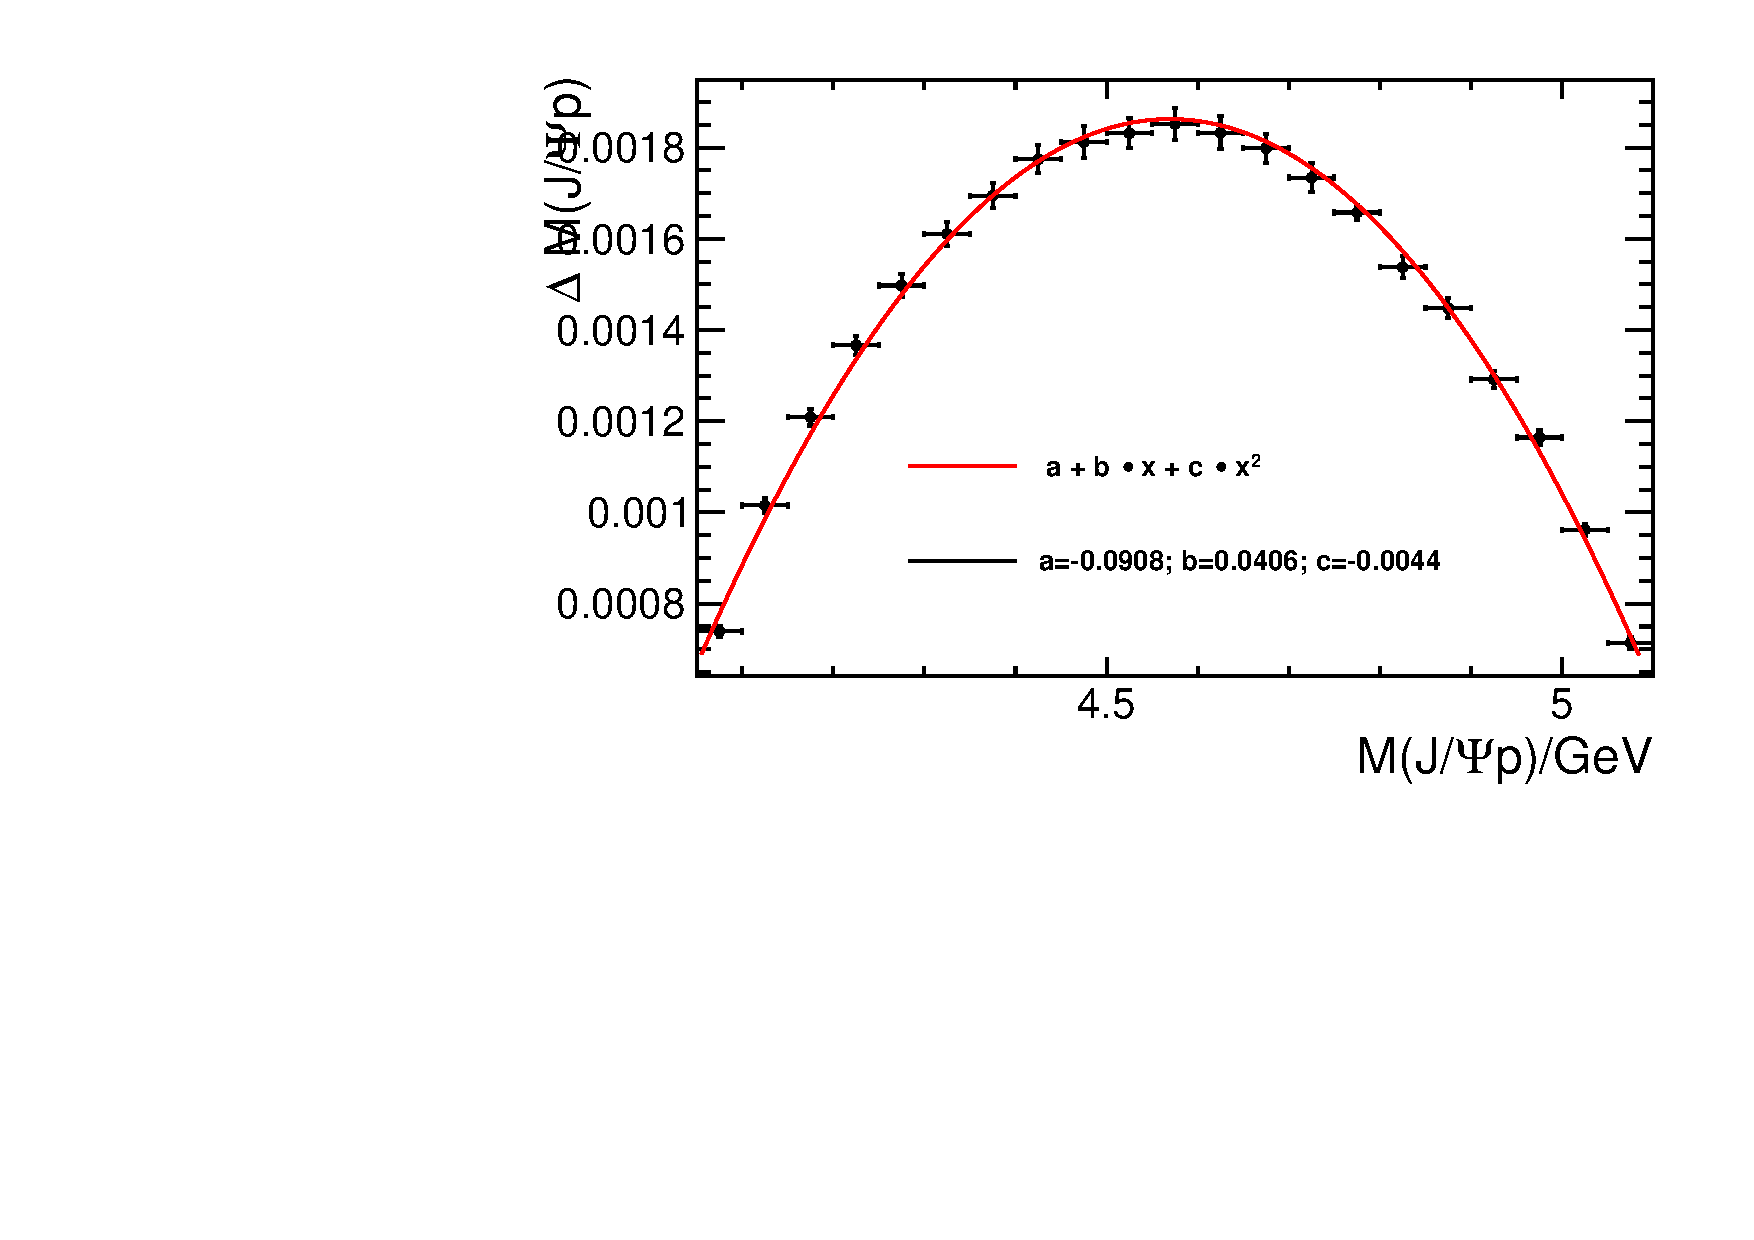
\includegraphics[width=0.5\textwidth]{Figures/08_JpsipK/plot_mass_res/run2}%
   \caption{The $m_{\jpsi\proton}$ resolution dependented on the mass itself.}
\label{fig:Mass_res_jpsip}
\end{figure}










